\section{Quantitative Evaluation: Machine vs. Human Quality Scores} 

In this experiment, we test whether sentence-level quality scores for MT text can improve users' ability to identify translated text that is untrustworthy and should be re-translated by a human. We test VeriCAT with ground truth quality scores generated by humans against VeriCAT with QE model scores. The following sections outline the study in more detail. 

\subsection{XAI Techniques} 

XAI Technique is a between-subjects factor in this experiment. As controls, we test a baseline condition with no XAI, a condition in which ground truth quality scores generated by humans are shown alongside MT text, and an experimental condition in which QE scores are shown alongside MT text. This results in a 3 condition experiment (No XAI, Human Quality, and Predicted Quality). We include the Human Quality condition in an effort to isolate user performance issues due to ambiguous quality scores from performance issues due to quality scores in general. In other words, because the QE model is not perfect we included a ``perfect" version of VeriCAT to gather whether quality scores could improve user performance even in the best case. Examples of stimuli are shown in Figure \ref{fig:exp_stim}. The Human Quality and Predicted Quality conditions are described in more detail below.  
 

\begin{compacthang}
    \item \textbf{Human Quality scores} These scores range from 0 to 100 with 0 indicating a poor quality translation, and 100 indicating a perfect translation. Scores are shown to users as percentages and progress bars, as shown in Figure \ref{fig:p1_human_quality}. We included only sentences with clearly good (> 70) or poor (< 30) quality scores, and used scores generated by humans \ab{need to add correct name}. We included only scores above 70 or below 30 to avoid the confounding factor of no clear difference between high and low sentence-level quality estimations. We include this condition, because predicted scores are not always sufficiently differentiated between high and low and we wanted to see if in the best case (i.e. with highly discriminate scores) quality scores can improve user performance.  

    \item \textbf{Predicted Quality scores} These scores are identical to the Human Quality scores in their range and presentation by VeriCAT. Unlike the ground truth scores used in the Human Quality condition, these scores are generated by a QE model and are therefore imperfect. Our goal in including predicted quality scores alongside ground truth scores is to understand how they perform in comparison to ground truth scores. Figure \ref{fig:p3_predicted_quality} shows an example of this condition. One notable difference between these scores and the Human Quality scores is that the magnitude of difference between high and low scores is much smaller for Predicted Quality scores.   
    
\end{compacthang}

\subsection{Passage Type}
We postulate that without XAI users will rely on fluency as a proxy for translation quality. Prior work has shown that this is the case when it comes to trust of MT \cite{martindaleFluency2018}. However, there are cases where this technique fails. For example, sentences written in ALL CAPS are notoriously difficult for MT, and often what they are translated is inaccurate but deceptively fluent. 

Each sentence can fall into one of four categories: poor fluency + poor quality, poor fluency + good quality, good fluency + poor quality, good fluency + good quality. Of these, we expect  sentences in the good fluency + poor quality, and poor fluency + good quality categories to be the most difficult for participants to assess. To test if these different sentence types have an effect on participants’ performance we arrange two different types of passages. 

\begin{compacthang}
    \item \textbf{Type 1} Good fluency + good quality, good fluency + poor quality, poor fluency + good quality. In this passage type we expect participants assigned to baseline (no XAI) to select the poor fluency sentence for re-translation. This passage type is designed to test if participants in an XAI condition will follow the quality indicators shown by the XAI to select a sentence for re-translation, or if they will also use fluency to decide. Passage 1 as shown in Figure \ref{fig:p1_human_quality} is of this type.    

    \item \textbf{Type 2} Good fluency + good quality, poor fluency + good quality, poor fluency + poor quality. In this passage type we expect participants assigned to baseline (no XAI) to select one of the poor fluency sentences for re-translation. This passage type is designed to test if participants in an XAI condition will follow the quality indicators shown by the XAI to select a sentence for re-translation (particularly because it should help them choose which poor fluency sentence to select), or if they will also use fluency to decide. Passage 3 as shown in Figure \ref{fig:p3_predicted_quality} is of this type.     
\end{compacthang}

\begin{figure}
    \centering
    
    \begin{subfigure}[t]{0.45\textwidth}
        \centering
        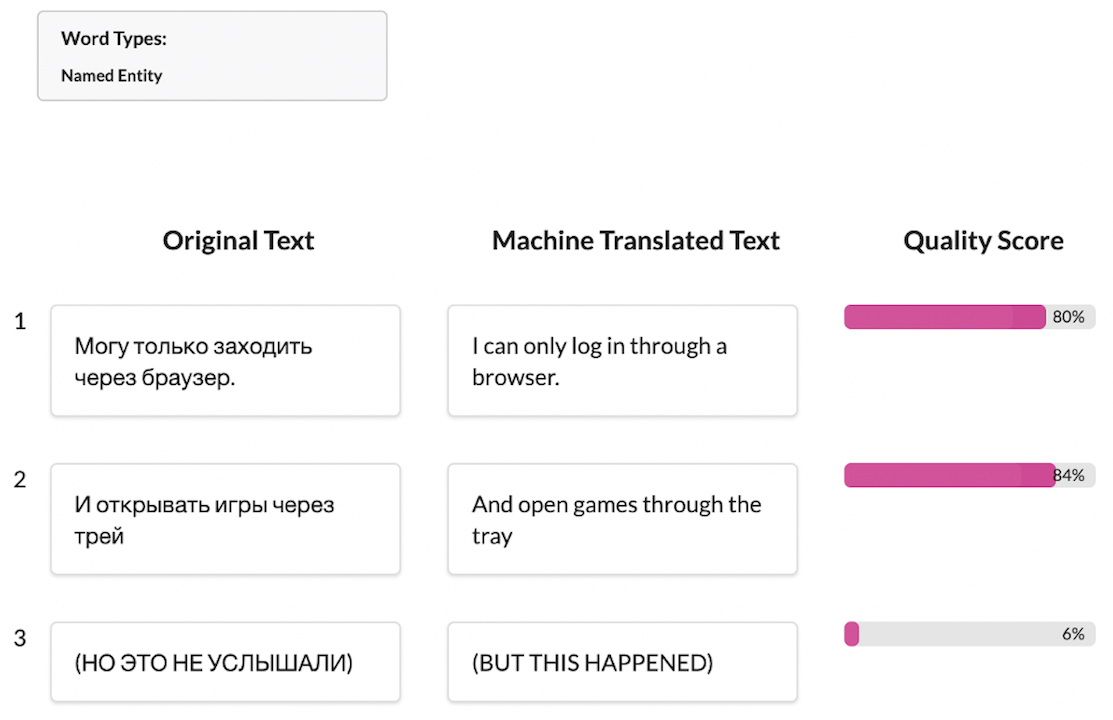
\includegraphics[width=\linewidth]{p1_v_0.png} 
        \caption{Passage 1 (passage type 1), Human Quality condition} \label{fig:p1_human_quality}
    \end{subfigure}
    \hfill
     \begin{subfigure}[t]{0.45\textwidth}
        \centering
        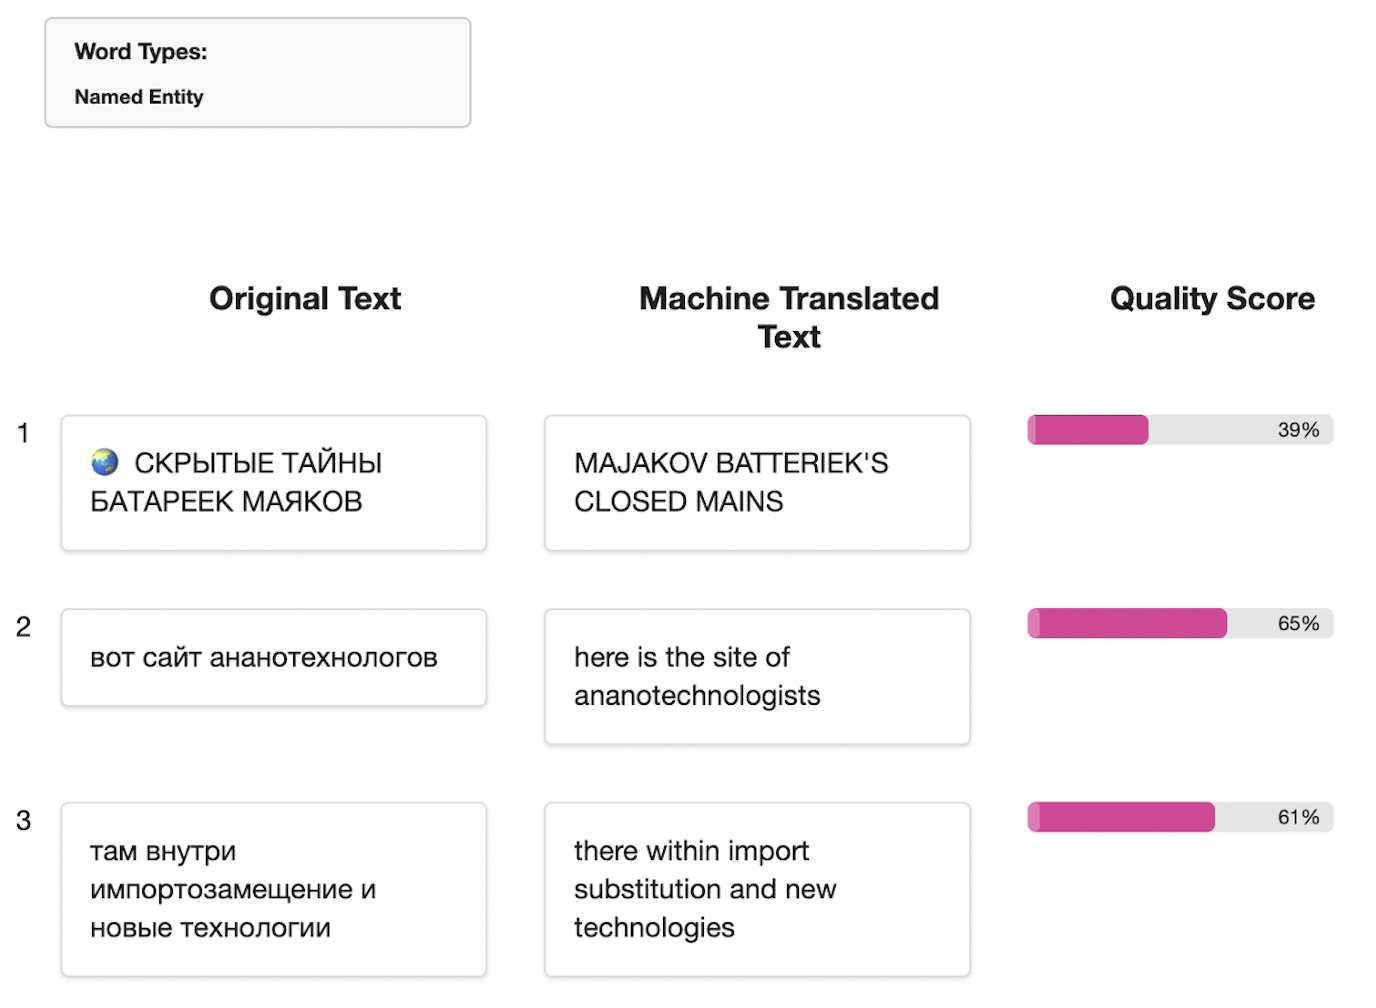
\includegraphics[width=\linewidth]{p3_p_0.png} 
        \caption{Passage 3 (passage type 2), Predicted Quality condition} \label{fig:p3_predicted_quality}
    \end{subfigure}
    
    \caption{Select examples of stimuli. All stimuli are available in supplemental materials.}
    \label{fig:exp_stim}
    
\end{figure}

\subsection{Task} 
We run a 3 condition experiment where each condition consists of a different XAI technique. Within each condition we include 2 passages of type 1 followed by 2 of type 2. The experimental task aimed to replicate the Facebook “Does this need a human translation?” situation as closely as possible within a controlled setting. For each passage the user is asked to look at the passage of text (comprised of 3 sentences), decide if any of the sentences in the passage should be re-translated by a human, and then answer 2 information retrieval questions based on the passage. The prompt before each passage is as follows:

\begin{quote}
Below is a passage written in Russian with an English translation generated by artificial intelligence. When you are ready, you will be asked to answer two comprehension questions. \textbf{You may select up to one section of the passage for re-translation by a human.} We recommend selecting the section you judge to have the poorest machine translation for re-translation by a human. 

Click ``I’m ready to see the questions'' when you are ready to see the comprehension questions. \textbf{If you would like a human re-translation of any section of the passage you must request it BEFORE you click ``I’m ready to see the questions''.} Once you click ``I’m ready to see the questions'', comprehension questions will appear on the page alongside the Russian test, English Machine translation, and any human translations you requested.  
\end{quote}

Participants were then given the chance to select sentence 1, 2, or 3 of the passage for re-translation by a human, or no-retranslation. After their selection the original passage and machine translation remained on the screen in addition to the human translation of whichever sentence they selected for re-translation, and two information retrieval questions. 

\begin{table}[]
\resizebox{0.60\textwidth}{!}{%
\begin{tabular}{c|c|c}
\hline
\begin{tabular}[c]{@{}c@{}}Human Quality Score XAI\\ (Human Quality)\end{tabular} & \begin{tabular}[c]{@{}c@{}}Predicted Quality Score XAI\\ (Predicted Quality)\end{tabular} &  \begin{tabular}[c]{@{}c@{}}No XAI\\ (No XAI)\end{tabular} \\ \hline
                                                                    59                                                                       & 59                                                                                         & 47                                                        \\ \hline
\end{tabular}
}
\caption{N for each condition. }
\label{tab:exp_N}
\end{table}

\subsection{Participants} 

We recruited 193 participants from Amazon Mechanical Turk. Participation was restricted to
workers in the United States with an approval rating of greater than 90 percent. Participants were paid a base rate of USD $1.60$ for participation. Before analysis, participants who answered information retrieval questions for passage 1 and passage 2 incorrectly (which were attention check questions) were dropped from analysis ($N = 28$).  This left $N = 165$ participants distributed among stimuli as shown in Table \ref{tab:exp_N}. Demographics of participants are shown in Table \ref{tab:exp_demo}.


\begin{table}[h!]
\begin{threeparttable}[b]
\begin{tabular}{ll}
\hline
N                                                                                & 165                                                                                                                                                    \\ \hline
Age                                                                              & \begin{tabular}[c]{@{}l@{}}18-24: 6.7\%, 25-34: 45.5\%, 35-44: 24.8\%, \\ 45-54: 14.5\%, 55-64: 7.3\%, 65+: 1.2\%\end{tabular}                                     \\ \hline
Gender                                                                           & \begin{tabular}[c]{@{}l@{}}Female: 38.2\%, Male: 61.2\%, Non-binary: 0.6\%\end{tabular}                                                             \\ \hline
Education                                                                        & \begin{tabular}[c]{@{}l@{}}High School: 13.3\%, Associates: 12.1\%, Bachelors: 60.0\%, \\ Masters: 11.5\%, Professional: 2.4\%, Doctorate: 0.6\%\end{tabular}                            \\ \hline
\end{tabular}
\end{threeparttable}
\caption{Participant demographics.}
\label{tab:exp_demo}
\end{table}

\subsection{Procedure}

The experiment followed an approved protocol per redacted\_for\_anonymity’s company policy, and was posted as a HIT on Amazon Mechanical Turk. Workers who accepted the HIT followed a link to the experiment. After providing informed consent, participants were taken to an instruction page explaining the experiment. This page explained that they would see 4 passages of text translated from Russian to English by AI. They were told that they would be asked to answer two comprehension questions for each passage, but before doing so would have the opportunity to see one of the sentences in the passage re-translated by a human. After the instruction page, participants were shown the four passages one at a time. Participants could take as much time with each stimulus as they wanted before clicking a button to select which section of the passage they wanted re-translated by a human and viewing the questions to answer. After completing the main task participants were asked to complete a short post-experiment questionnaire, the Tolerance for Ambiguity Survey from Geller et al. 1993 \cite{gellerTolerance1993}, a short demographic questionnaire, and to provide any additional feedback they wished.

\subsection{Hypotheses}

%We postulate that providing quality estimations for each sentence will help participants identify the sentence of lowest quality for re-translation only in cases where there is a significant difference between scores. In other words, we expect participants in the Human Quality condition to perform significantly better than participants in the Predicted Quality condition. 

To evaluate the VeriCAT system with Human vs Predicted Quality Scores, we test the following hypotheses:

\begin{compacthang}
    \item \textbf{H1}: Participants in the XAI conditions will have higher accuracy in identifying which sentence in a passage is of low quality and should be re-translated than participants in other two conditions. 
    \item \textbf{H2}: Participants in the XAI conditions will have a greater change in trust of machine translation than participants in the No XAI condition. 
    \item \textbf{H3}: Participants’ tolerance for ambiguity will correlate with how well they are able to use the Predicted Quality XAI to perform the experimental task. 
    \item \textbf{H4}: Participants’ experience using machine translation will correlate with how well they are able to use XAI to perform the experimental task. 
    \item \textbf{H5}: Participants’ self-rated expertise in AI, MT, visualization, and statistics will correlate with how well they are able to use XAI to perform the experimental task.   
\end{compacthang}

\subsection{Findings}

We consider a participant’s answer correct if they select the sentence in a passage with the lowest quality score as the one to get re-translated by a human. To calculate overall accuracy, we sum the number of correct answers across all four passages and divide by 4. The following analyses use this outcome measure to test the hypotheses listed above.

\subsubsection{Does XAI help?}

We start by looking at which sentences people chose to re-translate for each condition and passage. For all  passages we see participants in both Quality conditions are on average most accurate at selecting the correct sentence for re-translation. The proportions of participants selecting the correct sentences for re-translation in the Predicted quality condition is less than that of the Human Quality condition, but still far higher than the No XAI condition. Interestingly, we see that participants in the No XAI condition tend to opt for no-retranslation, or re-translating a poor fluency sentence. Proportions of participants giving each answer for each passage and condition are shown in Figure \ref{fig:exp_prop_answers}.

\begin{figure}*
    \centering
    
    \cbox{bar-noXai} \textit{No XAI} \quad
    \cbox{bar-Qual} \textit{Human Quality} \quad
    \cbox{bar-PredictQ} \textit{Predicted Quality} \quad
    
    \begin{subfigure}[t]{0.45\textwidth}
        \centering
        \scalebox{0.7}{
        \begin{bchart}[step=.25,max=1,width=\linewidth]
        \bcbar[color=bar-noXai]{.06}
        \bclabel{\textit{Good Fluency}}
        \bcbar[color=bar-Qual]{.51}
        \bclabel{\textit{Poor score}}
        \bcbar[color=bar-PredictQ]{.37}
        \bcskip{6pt}
        
        \bcbar[color=bar-noXai]{.15}
        \bclabel{\textit{Good Fluency}}
        \bcbar[color=bar-Qual]{.15}
        \bclabel{\textit{Good score}}
        \bcbar[color=bar-PredictQ]{.07}
        \bcskip{6pt}
        
        \bcbar[color=bar-noXai]{.38}
        \bclabel{\textit{Poor Fluency}}
        \bcbar[color=bar-Qual]{.14}
        \bclabel{\textit{Good score}}
        \bcbar[color=bar-PredictQ]{.31}
        \bcskip{6pt}
        
        \bcbar[color=bar-noXai]{.40}
        \bclabel{\textit{No}}
        \bcbar[color=bar-Qual]{.20}
        \bclabel{\textit{Re-translation}}
        \bcbar[color=bar-PredictQ]{.25}
        
        \bcxlabel{Proportion of Participants Selecting}
        \end{bchart}}
        \caption{Passage 1} 
        \label{fig:exp_p1_prop_answers}
    \end{subfigure}
    \hfill
    \begin{subfigure}[t]{0.45\textwidth}
        \centering
        \scalebox{0.7}{
        \begin{bchart}[step=.25,max=1,width=\linewidth]
        \bcbar[color=bar-noXai]{.06}
        \bclabel{\textit{Good Fluency}}
        \bcbar[color=bar-Qual]{.53}
        \bclabel{\textit{Poor score}}
        \bcbar[color=bar-PredictQ]{.37}
        \bcskip{6pt}
        
        \bcbar[color=bar-noXai]{.13}
        \bclabel{\textit{Good Fluency}}
        \bcbar[color=bar-Qual]{.12}
        \bclabel{\textit{Good score}}
        \bcbar[color=bar-PredictQ]{.08}
        \bcskip{6pt}
        
        \bcbar[color=bar-noXai]{.21}
        \bclabel{\textit{Poor Fluency}}
        \bcbar[color=bar-Qual]{.15}
        \bclabel{\textit{Good score}}
        \bcbar[color=bar-PredictQ]{.20}
        \bcskip{6pt}
        
        \bcbar[color=bar-noXai]{.60}
        \bclabel{\textit{No}}
        \bcbar[color=bar-Qual]{.20}
        \bclabel{\textit{Re-translation}}
        \bcbar[color=bar-PredictQ]{.34}
        
        \bcxlabel{Proportion of Participants Selecting}
        \end{bchart}}
        \caption{Passage 2} 
        \label{fig:exp_p2_prop_answers}
    \end{subfigure}
    \hfill
     \begin{subfigure}[t]{0.45\textwidth}
        \centering
        \scalebox{0.7}{
        \begin{bchart}[step=.25,max=1,width=\linewidth]
        \bcbar[color=bar-noXai]{.26}
        \bclabel{\textit{Poor Fluency}}
        \bcbar[color=bar-Qual]{.69}
        \bclabel{\textit{Poor score}}
        \bcbar[color=bar-PredictQ]{.68}
        \bcskip{6pt}
        
        \bcbar[color=bar-noXai]{.19}
        \bclabel{\textit{Poor Fluency}}
        \bcbar[color=bar-Qual]{.05}
        \bclabel{\textit{Good score}}
        \bcbar[color=bar-PredictQ]{.15}
        \bcskip{6pt}
        
        \bcbar[color=bar-noXai]{.09}
        \bclabel{\textit{Good Fluency}}
        \bcbar[color=bar-Qual]{.10}
        \bclabel{\textit{Good score}}
        \bcbar[color=bar-PredictQ]{.03}
        \bcskip{6pt}
        
        \bcbar[color=bar-noXai]{.47}
        \bclabel{\textit{No}}
        \bcbar[color=bar-Qual]{.15}
        \bclabel{\textit{Re-translation}}
        \bcbar[color=bar-PredictQ]{.14}
        
        \bcxlabel{Proportion of Participants Selecting}
        \end{bchart}}
        \caption{Passage 3} 
        \label{fig:exp_p3_prop_answers}
    \end{subfigure}
    \hfill
    \begin{subfigure}[t]{0.45\textwidth}
        \centering
        \scalebox{0.7}{
        \begin{bchart}[step=.25,max=1,width=\linewidth]
        \bcbar[color=bar-noXai]{.45}
        \bclabel{\textit{Poor Fluency}}
        \bcbar[color=bar-Qual]{.64}
        \bclabel{\textit{Poor score}}
        \bcbar[color=bar-PredictQ]{.64}
        \bcskip{6pt}
        
        \bcbar[color=bar-noXai]{.02}
        \bclabel{\textit{Poor Fluency}}
        \bcbar[color=bar-Qual]{.12}
        \bclabel{\textit{Good score}}
        \bcbar[color=bar-PredictQ]{.08}
        \bcskip{6pt}
        
        \bcbar[color=bar-noXai]{.11}
        \bclabel{\textit{Good Fluency}}
        \bcbar[color=bar-Qual]{.10}
        \bclabel{\textit{Good score}}
        \bcbar[color=bar-PredictQ]{.12}
        \bcskip{6pt}
        
        \bcbar[color=bar-noXai]{.43}
        \bclabel{\textit{No}}
        \bcbar[color=bar-Qual]{.14}
        \bclabel{\textit{Re-translation}}
        \bcbar[color=bar-PredictQ]{.15}
        
        \bcxlabel{Proportion of Participants Selecting}
        \end{bchart}}
        \caption{Passage 4} 
        \label{fig:exp_p4_prop_answers}
    \end{subfigure}
    
    \caption{Proportions of participants selecting each type of sentence for re-translation by passage.}
    \label{fig:exp_prop_answers}

\end{figure}

To test if the differences we observe are significant we ran a Kruskal-Wallis test of $overall\_score \sim condition$ \footnote{We use a Kruskal-Wallis test because according to the Shapiro-Wilk Normality test overall\_score is not normally distributed ($W = 0.87, p < 0.001$).} and find a significant difference across conditions ($H(2) = 29.7, p < 0.001$). A post-hoc Dunn’s multiple comparisons test with a Bonferroni corrected alpha ($\alpha = 0.02$) shows significant pairwise differences between Human Quality and No XAI ($Z = 5.2, p < 0.01$), and No XAI and Predicted Quality ($Z = -4.3, p < 0.01$). Figure \ref{fig:exp_overall_distribution} shows overall\_score distributions by condition. 

\begin{figure}[h!]
    \centering
    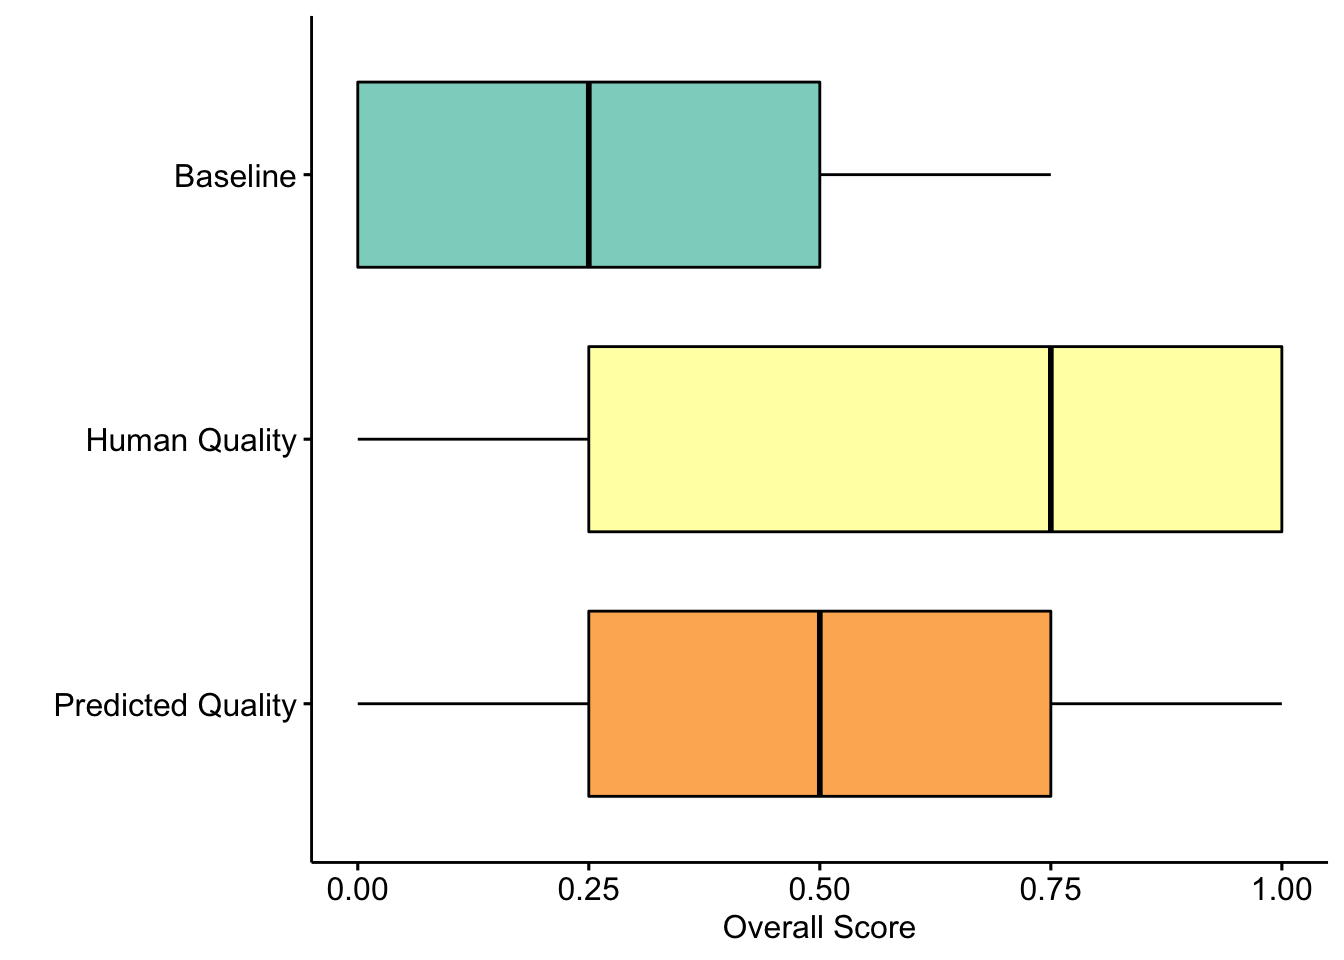
\includegraphics[width=0.50\textwidth]{exp2_overall_distribution.png}
    \caption{Boxplot of overall score by condition.}
    \label{fig:exp_overall_distribution}
\end{figure}

These results suggest that showing sentence-level quality scores can significantly improve participants’ performance over No XAI, regardless of if they are human generated or model predictions. Therefore, we \textbf{accept H1}. The results also show that there is no significant difference in performance between human and predicted quality scores, suggesting that though imperfect, predicted quality scores are as effective as human generated quality scores. 

\subsubsection{Does XAI affect trust?}

We asked participants before the experimental task “Please rate how much you trust artificial intelligence to correctly translate sentences from a language you do not speak into a language you do speak from 1 (No trust) to 5 (Complete trust).”  We asked the same question at the end of the experimental task. To analyze whether different conditions changed participant’s trust in machine translation, we calculated delta\_trust for each participant by subtracting their answer to the pre-experimental task trust question from their answer to the post-experimental task trust question. 

We run a Kruskal-Wallis test of delta\_trust $\sim$ condition \footnote{We use a Kruskal-Wallis test because according to the Shapiro-Wilk Normality test delta_trust is not normally distributed ($W = 0.74, p < 0.001$).} and find no significant difference across conditions ($H(2) = 3.5, p = 0.17$). This suggests that neither the presence of XAI nor the different types of quality scores significantly affected participants’ trust in machine translation, thus we \textbf{reject H2}. Average change in trust by condition is shown in Figure \ref{fig:exp_delta_trust}.

\begin{figure}[h!]
    \centering
    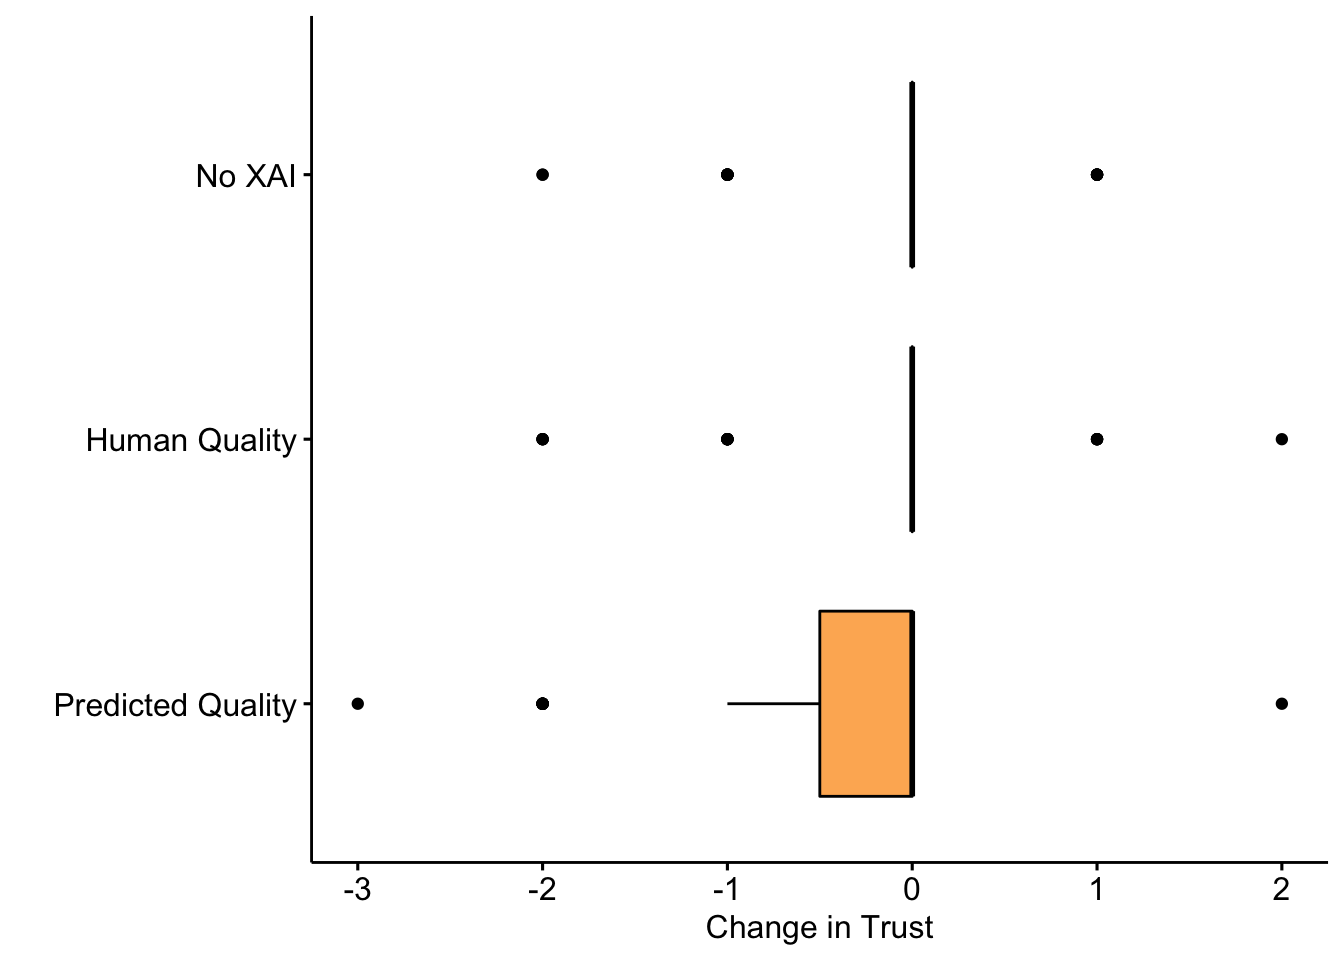
\includegraphics[width=0.50\textwidth]{exp2_delta_trust.png}
    \caption{Boxplot of change in trust by condition.}
    \label{fig:exp_delta_trust}
\end{figure}

\subsubsection{Is the efficacy of XAI influenced by participants' individual differences?}

Prior work has shown that individual user differences can play a strong role in how well users utilize a visualization for a problem solving task\cite{liuSurvey2020}. However, there has been little research investigating how individual differences can affect understanding, trust, and use of AI. In an effort to start answering this question we captured three different individual differences of users (intolerance for ambiguity, usage of MT, and self-rated expertise) and analysed whether there were any correlations between these measures and users’ overall\_score. Our findings follow.

\paragraph{Intolerance for Ambiguity} 

Given the survey instrument we use to measure Intolerance for Ambiguity\cite{gellerTolerance1993} participants’ scores could range from 7 (extremely low intolerance for ambiguity) to 49 (extremely high intolerance for ambiguity). The median score for intolerance for ambiguity of participants is 30. 

Within each condition we tested for a significant Pearson correlation between participants’ overall\_score and intolerance\_for\_ambiguity. Regression lines for each condition are shown in Figure \ref{fig:exp_intol_ambiguity}. We find no significant correlation in any condition (Human Quality -- ($r(57) = -0.14, p = 0.29$), Predicted Quality --  ($r(57) = 0.03, p = 0.81$), No XAI -- ($r(45) = -0.01, p = 0.95)$). This suggests that intolerance for ambiguity has no effect on participants' performance, thus we \textbf{reject H3}. 

\begin{figure}[h!]
    \centering
    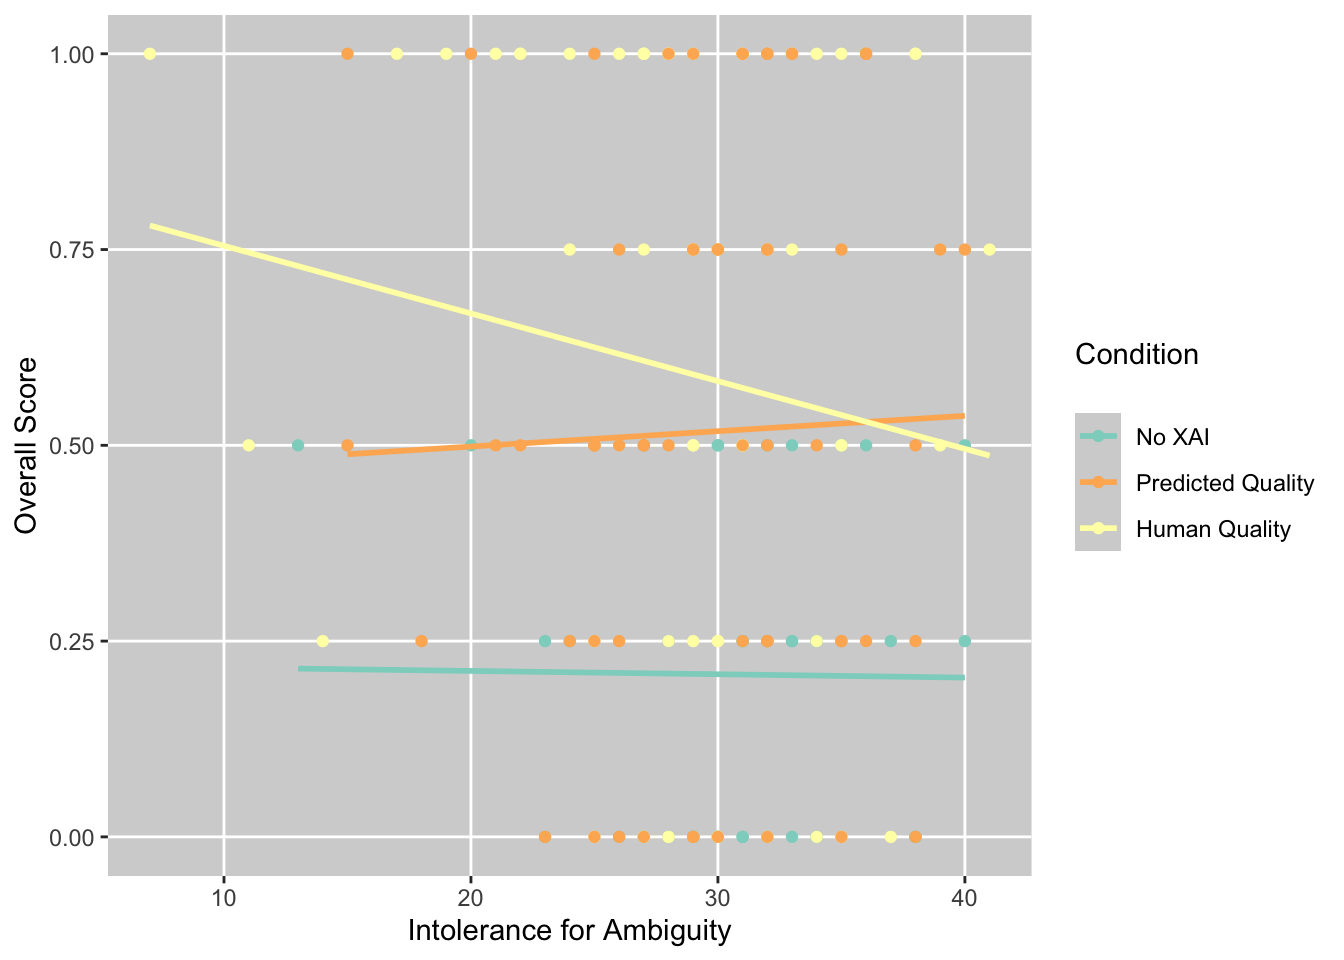
\includegraphics[width=0.50\textwidth]{exp2_intol_ambiguity.png}
    \caption{Regression lines of overall score and intolerance for ambiguity by condition.}
    \label{fig:exp_intol_ambiguity}
\end{figure}

\paragraph{Usage of Machine Translation} 
We ask participants to rank how often they use Google Translate and Facebook Translate on a five-point scale of Never, Yearly, Monthly, Weekly, Daily. We assign weights to each point in the scale ranging from 1 (Never) to 5 (Daily) and use these to calculate a machine translation usage score for each participant. The higher this score, the more often a participant indicated using MT. 

Within each condition we test for a Pearson correlation between participants’ frequency of MT usage and performance. Regression lines for each condition are shown in Figure \ref{fig:exp_MT_use}. We find a significant correlation between frequency of MT usage and overall score for participants in the Human Quality condition ($r(57) = -0.32, p < 0.05$), and no significant correlation in any other condition (Predicted Quality -- ($r(57) = -0.21, p = 0.11$), No XAI -- ($r(45) = -0.23, p = 0.11$)). This suggests that in the Human Quality condition as participants’ frequency of MT usage increases, their performance decreases, thus we \textbf{partially accept H4}.

\begin{figure}[h!]
    \centering
    \includegraphics[width=0.50\textwidth]{exp2_MT_use.png}
    \caption{Regression lines of overall score and frequency of MT usage by condition.}
    \label{fig:exp_MT_use}
\end{figure}

\paragraph{Self-rated Expertise}

We ask participants to rate their own expertise from 1 (Novice) to 5 (Expert) in four areas related to XAI: AI, MT, visualization, and statistics. We use these self ratings to test for correlations between participants’ self-rated expertise and performance. Regression lines for each condition are shown in Figure \ref{fig:exp_expert}.  

\begin{figure}[h!]
    \centering
    
    \cbox{bar-noXai} \textit{No XAI} \quad
    \cbox{bar-Qual} \textit{Human Quality} \quad
    \cbox{bar-PredictQ} \textit{Predicted Quality} \quad
    
    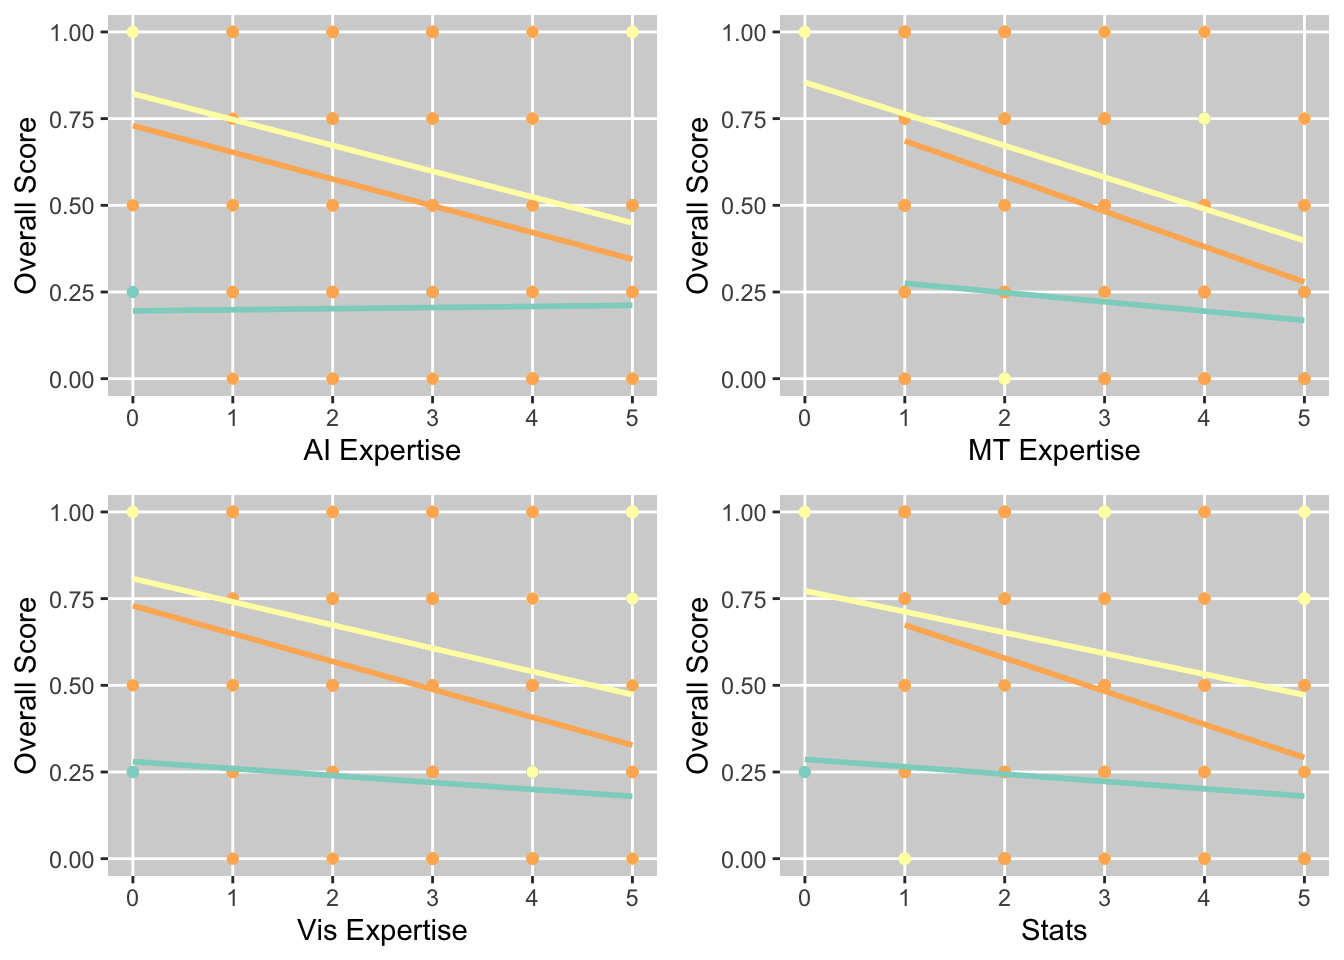
\includegraphics[width=0.50\textwidth]{exp2_expert.png}
    \caption{Regression lines of overall score and self-rated expertise by condition.}
    \label{fig:exp_expert}
\end{figure}

Within each condition we test for a Pearson correlation between each self-rated expertise and overall score. In the Human Quality, and Predicted Quality conditions we find a significant correlations between self rated expertise in AI and MT and overall score. In addition, we find significant correlations between self-rated expertise in visualization and statistics and overall score in the Predicted Quality condition.  
(Analysis results for all of these tests are listed in Table \ref{tab:exp1_expertise_stats}.) Overall, our results suggest that in all cases except for No XAI as self-rated expertise in AI and MT (and in the case of Predicted Quality visualization and statistics) increase, overall score decreases, thus we \textbf{accept H5}.

\begin{table}[]
\resizebox{0.70\textwidth}{!}{%
\begin{tabular}{llc}
\hline
\multicolumn{1}{c}{Measure}                            & \multicolumn{1}{c}{Condition} & Result                                   \\ \hline
\multirow{4}{*}{Self-rated expertise in AI}            & Human Quality              & \textbf{r(57) = -0.27, p \textless 0.05} \\
                                                       & Predicted Quality          & \textbf{r(57) = -0.29, p \textless 0.05}         \\
                                                       & No XAI                     & r(45) = 0.02, p = 0.91                   \\ \hline
\multirow{4}{*}{Self-rated expertise in MT}            & Human Quality              & \textbf{r(57) = -0.31, p \textless 0.05} \\
                                                       & Predicted Quality          & \textbf{r(57) = -0.40, p \textless 0.01}          \\
                                                       & No XAI                     & r(45) = -0.13, p = 0.39                  \\ \hline
\multirow{4}{*}{Self-rated expertise in visualization} & Human Quality              & r(57) = -0.24, p = 0.06                  \\
                                                       & Predicted Quality          & \textbf{r(57) = -0.31, p \textless 0.05}                  \\
                                                       & No XAI                     & r(45) = -0.11, p = 0.48                  \\ \hline
\multirow{4}{*}{Self-rated expertise in statistics}    & Human Quality              & r(57) = -0.21, p = 0.10                  \\
                                                       & Predicted Quality          & \textbf{r(57) = -0.36, p \textless 0.01}          \\
                                                       & No XAI                     & r(45) = -0.11, p = 0.46                  \\ \hline
\end{tabular}%
}
\caption{Pearson correlation results for each self-rated expertise measure by condition. Significant results are in \textbf{bold}.}
\label{tab:exp1_expertise_stats}
\end{table}

\subsection{Discussion of Findings} 

The purpose this experiment was to test if imperfect machine-generated sentence-level quality scores could improve user performance in identifying poor quality machine translations as well as human-generated sentence-level quality scores. We find that although user performance is slightly lower with machine-generated quality scores, there is no significant difference in performance compared to human-generated quality scores. Moreover, we find that both machine- and human-generated quality scores significantly improve user performance compared to no XAI. 
Moreover, we find Predicted Quality scores have no effect on participants' trust of MT, nor does participants' intolerance for ambiguity affect their ability to effectively use predicted quality scores. Unlike participants in the Human Quality condition, we find no significant correlation between participants' overall score and frequency of MT use in the Predicted Quality condition. Similar to the Human Quality condition, we find a significant negative correlation between participants' self-rated expertise and overall score in the Predicted Quality condition.     

All of these findings suggest that although the model for machine-generated sentence-level quality scores is not perfect it currently performs well enough to be used as a part of MT XAI, and doing so will not introduce any additional burdens to different types of users. In fact, utilizing Predicted Quality scores instead of Human Quality scores may remove the potentially negative effect of prior MT usage on performance.  


